\documentclass[10pt,twocolumn]{article}

\usepackage{times}
\usepackage{fullpage}
\usepackage{listings}

\begin{document}

\title{\bf Detecting RCU bugs}
\author{Dhaval Giani and Akshay Kumar}
\date{}
\maketitle
\thispagestyle{empty}

\lstset{language=C,basicstyle=\ttfamily,tabsize=4, columns=fullflexible}
\begin{abstract}
Application debugging is a tedious chore in software development cycle. The need of an efficient debugger increases with the complexity of software involving parallel system. Read Copy Update (RCU) is a wait-free synchronization mechanism which gets heavily used in the parallel system to reduce overheads and avoid deadlocks. Being complex in its design, one needs to take a lot of care while using RCU. The incorrect usage of RCU often leads to programming error or bugs. The existing solution for analysing such bugs are imprecise and generate false positive. 

In this project we introduces a new approach for analysing such bugs using \emph{Software Watchpoint}. Our \emph{Watchpoint} mechanism is implemented using Dynamic Binary Instrumentation (DBI) technique and provides efficient infrastructure to enforce memory access policy. We used \emph{Watchpoint} to track and verify the references of RCU protected data. Our system is precise and imposes moderate overhead for reader and low overhead for writer thread. Our system is limited in its approach and identify bugs related to pointer leak in classical RCU. 

\end{abstract}

\section{Introduction}\label{sec:intro}
Parallel programming is already mainstream these days. There are a wide variety
of mechanisms being used to provide synchronization and serialization.
Operating systems are a popular example for utilizing various synchronization
mechanims%Add citations here for spinlocks, mutexes and for RCU, with possibly links to the sourcse as opposed to publications for Linux/BSD/Solaris
With scalability being extremely important for the Operating Systems,
techniques have been proposed to reduce the overheads by utilizing lock-free
techniques. Read Copy Update~\cite{paulmck:TechReport} is one such technique which is
heavily used in the Linux Kernel. RCU has been described as a publish-subscribe
technique.

In its simplest form, readers do absolutely nothing when they enter or exit an
RCU read critical section. On the other hand updaters synchronize with the use
of one of the traditional mechanisms such as spin locks or mutexes while updating.
Following an update, any new readers gets to access the updated version. However
readers who came in before the update was `published` would still be guaranteed
to the see the older version which is reclaimed only after all the pre-existing
readers have gone away.

RCU is becoming increasingly relevant today with a userspace implementation also
being released and used.%cite urcu paper and the flocking using RCU paper


\section{Background}\label{sec:back}
Programming with RCU is a completely different paradigm as compared to traditional
synchronization techniques. Similar to other techniques, the programmer must take care to clearly define
read critical sections. However, on the update side, the programmer must use another
traditional synchronization technique. We further illustrate difference with the
use of two examples.

\begin{figure}[t]
\centering
\begin{lstlisting}
rwlock_t q_lock;
global datatype *q;

f() {
	...
	rwlock_read_lock(&q_lock);
	do_something(q);
	rwlock_read_unlock(&q_lock);
	...
}
\end{lstlisting}
\caption{Using Reader Writer locks}\label{fig:rwuse}
\end{figure}

\begin{figure}[b]
\centering
\begin{lstlisting}
global datatype *q;

f() {
	dataype *p;
	...
	rcu_read_lock();
	p = rcu_dereference(q);
	do_something(p);
	rcu_read_unlock();
	...
}
\end{lstlisting}
\caption{Using RCU}\label{fig:RCUuse}
\end{figure}

Figure~\ref{fig:rwuse} shows how a
typical Reader Writer lock works. \emph{q} is the shared data which various readers
and writers wish to access. \emph{q\_lock} is used to synchronize access to \emph{q}.
First the reader locks the rwlock, \emph{q\_lock},
in the read mode. It then goes ahead an reads the data in \emph{q}. Finally once it is
done, it unlocks \emph{q\_lock}.

In contrast Figure~\ref{fig:RCUuse} gives an example of how RCU is used. \emph{q} is a global pointer
which points to some data which is protected with the use of RCU. When a reader
wishes to dereference that data, it first announces the beginning of an RCU critical
section using \emph{rcu\_read\_lock}. Then in order to derefence that data, it 
uses \emph{rcu\_dereference}. At this
point it holds a legal reference and RCU guarantees that structure will not be
reclaimed at least until this reader announces the end of the critical section.
The reader now proceeds to go ahead and use the reference it has. Finally once it
is done, it announces the end of a critical section with the use of \emph{rcu\_read\_unlock}.

The key difference to be noted is that while in the case of rwlocks, the readers
need to wait till they can lock the rwlock, RCU readers just announce the start
of a read critical section. In order to ensure that access is not interrupted,
a reference is obtained with the use of \emph{rcu\_dereference}. \emph{rcu\_dereference}
ensures that compiler optimizations which reorder access are prevented, as well
some prevent load store reordering on some architectures such as DEC Alpha.
Finally all accesses
to the shared data is through the use of \emph{p}. RCU guarantees that the data structure
will not be reclaimed till the reader announces the end of its critical section.

In order to aid further discussion, we now define two terms in context of RCU
\begin{itemize}
\item{\bf Quiescent State}: This is the state when a reader is not in an RCU read critical state.
\item{\bf Grace Period}: Any time period during which each thread has been observed in at least one quiescent state.
\end{itemize}

RCU has a list of well defined API. The most commonly used are
\begin{itemize}
\item\emph{rcu\_read\_lock}: Used to announce the beginning of a critical section.
\item\emph{rcu\_read\_unlock}: Used to announce the end of a critical section.
\item\emph{rcu\_dereference}: Used to obtain a reference to shared data
\item\emph{rcu\_assign\_pointer}: Used to announce an update.
\item\emph{synchronize\_rcu}: Used to wait till a grace period has passed.
\item\emph{call\_rcu}: Used to queue up a callback that takes place after the end of some grace period that starts in the future.
\end{itemize}


Using RCU requires careful attention from the programmer. There are some rules
and inherent assumptions while using RCU. For example, access to shared data
should only happen with a reference which has been obtained with the use of
\emph{rcu\_dereference}. This call should also happen only after an RCU read critical
section has announced. Any use of this reference obtained must be made before
this critical section ends. If a new critical section has been announced a
fresh reference must be obtained with the use of \emph{rcu\_dereference}. A quiescent
state (in some flavours of RCU) must only be announced once it has actually
taken place.~\footnote{It is also important to note that while care must be taken to announce a
quiescent state only when it has actually occured, one must not delay the announcement
of the quiescent state. Since RCU maintains multiple copies which are only reclaimed
after a grace period has occured, it serves only to increase the memory pressure on
the system.} On the update side, an update should only take place with use
of \emph{rcu\_assign\_pointer}. There are many other similar rules that must be
followed.


\section{Proposal}\label{sec:proposal}
As mentioned in Section~\ref{sec:back} usage of RCU requires a lot of care in
the use of RCU. There are many rules that must be followed while writing code
which uses RCU. Figures~\ref{fig:rcuderefbug} and~\ref{fig:rcuusebug} show
some examples.

\begin{figure}[h]
\centering
\begin{lstlisting}
f() {
	...
	rcu_read_lock();
	p = q;
	do_something(p);
	rcu_read_unlock();
	...
}
\end{lstlisting}
\caption{RCU bugs: Not using rcu\_derefence}\label{fig:rcuderefbug}
\end{figure}

\begin{figure}[h]
\centering
\begin{lstlisting}
f() {
	...
	rcu_read_lock();
	p = rcu_dereference(q);
	x = p;
	rcu_read_unlock();
	...
	rcu_read_lock();
	do_something(x);
	rcu_read_unlock();
	...
}
\end{lstlisting}
\caption{RCU bugs: Not using in the correct critical section}\label{fig:rcuusebug}
\end{figure}

In figure~\ref{fig:rcuderefbug} a reference to q takes place directly without the use
of \emph{rcu\_dereference}. In figure~\ref{fig:rcuusebug}, while p has been obtained with the
use of rcu\_dereference, it is used (in the form of x) after the critical section
has been announced. A similar bug would be if the reference obtained was outside the
critical section. These bugs can be broadly classed as RCU pointer leaks.

As mentioned in section~\ref{sec:back}, there are many rules that must be followed
while using RCU. For the purposes of this report, we shall name two rules.
\begin{itemize}
\item{\bf Rule 1}: Any reference to RCU protected must obtained with the use \emph{rcu\_dereference}
\item{\bf Rule 2}: Any reference obtained \emph{using rcu\_dereference} must be used with the critical section it was obtained in.
\end{itemize}

We shall call the bugs of the type represented in figure~\ref{fig:rcuderefbug} as \emph{Rule 1 violations}
and those in figure~\ref{fig:rcuusebug} as \emph{Rule 2 violations}.
This project aims to detect and report bugs of these two types.

Detecting these bugs is extremely challenging. Due to the nature of RCU implementation,
bugs are subtle and at times hard to reproduce. Even though the references have been
illegaly obtained, they might still be valid.

In order to detect \emph{Rule 1 violations}, we must first identify data
that has been protected by RCU. We must then be able to track every
dereference to it. We must also be in a position to instrument
every \emph{rcu\_dereference} call.

For \emph{Rule 2 violations}, we must know when a dereference takes place.
At that point in time, we need to be able to check if the reference has
been obtained legally. If so, we must know if it has been obtained in
the current critical section.

In order to detect these issues, we use \emph{generations}. \emph{Generations}
can be defined as an RCU critical section. A generation has the following
properties

\begin{itemize}

\item \emph{Generations} are per-thread
\item A new \emph{generation} starts when \emph{rcu\_read\_lock} is called
\item A \emph{generation} ends when \emph{rcu\_read\_unlock} is called

\end{itemize}

To detect these violations, we use \emph{granary} which is described in
further detail in section~\ref{sec:impl}. Granary provides us the ability
to add unlimited watchpoints.

We first identify RCU protected data.
This can be acheived in a number of ways. The easiest way is to intercept calls
to \emph{rcu\_assign\_pointer}. A watchpoint is added at that point. The watchpoint
is \emph{per-pointer}. The watchpoint is erased only when a reclaim takes place.

Whenever an \emph{rcu\_dereference} takes place, a check is made to confirm that
a \emph{generation} has started. If not, this detects that an \emph{rcu\_dereference}
has taken place outside a critical section and is a \emph{rule 2 violation} If a
generation has started, we then tag the associated RCU pointer with the current
generation.

When a dereference of RCU protected data takes place, the very first check is made
to see if a \emph{generation} has started. The absence of a generation detects
a \emph{rule 2 violation}.

Next the RCU pointer must be checked to see if it was legally obtained. This is checked by checking the
\emph{generation} information of the pointer. Since \emph{generation} information
is setup only at the point when an \emph{rcu\_dereference} takes place, absence
of this information indicates a \emph{rule 1 violations}.

However the presence of the \emph{generation} information does not imply that the RCU
pointer is legal. In order to confirm that, the \emph{generation} in the RCU pointer is
compared with current thread's \emph{generation}. If the two generations are the same,
then the RCU pointer is legal. Any other case denotes a \emph{rule 2 violation}


\section{Implementation Details}\label{sec:impl}
Section~\ref{sec:appr} discusses about the behavioural watchpoint and how they are important for debugging RCU based applications.
%our mechanism for implementing watchpoint for memory operations. We also described the details of shadow memory \& meta-information and how it can is used for tracking rcu synchronization primitive. 
This section describes about the implementation and the policies we used for tracking RCU primitives.

The design of our system, using Granary, is based on the consideration that it interposes at the kernel/module interface. While implementing our system we found that most of the  RCU primitives are defined as macro and inline functions~\cite{PaulEdwardMcKenneyPhD} which gets embedded into binary module. Granary being a DBI tool doesn’t know when one of these rcu interface function gets called. To handle this we annotated RCU primitives that gives a callbacks to kernel wrapper when these primitives is used. This is particularly helpful since it provided the infrastructure to track the usage of rcu primitive and update the contextual information. It is then used to check the violation of RCU rules and possible bugs. The different memory access policies we used to check the violation of RCU usage are as follows:

%The design of our system, using Granary, is based on the consideration that  
%One of the important challenge while implementing our system was most of the RCU primitives are defined as macro and inline functions~\cite{PaulEdwardMcKenneyPhD} which gets embedded into binary module. Granary being a DBI tool doesn’t know when one of these rcu interface function gets called. To handle this we annotated RCU primitives that gives a callbacks to kernel wrapper on its uses. This was particularly helpful since it provided the infrastructure to track the usage of rcu primitive and update the meta-information. The updated meta-information is then used to check the violation of RCU rules and possible bugs. The section below discusses the different memory access policy rcu protected data should follow and how meta-information is used to enforce them: 

\begin{enumerate}
\item[i)] \emph{Access of RCU protected data inside read critical section} To ensure the access of RCU protected data inside read critical section, the per-thread generation number should be even.% our system checks for the following policies: %uses thread and watchpoint \emph{generation number}.%. Before any memory read at watchpoint addresses our system checks both thread \& watchpoint \emph{Generation number} and ensures the following:
%	\begin {itemize}
%		\item[i)] Per-thread \emph{generation number} should be even to ensure the access of memory inside read critical section. %(\texttt{current\_thread\_info()$\rightarrow$spill\_slot[0]\%2 == 0})
		%\item[ii)] Per-object \emph{generation number} should be even and equal to thread \emph{generation number}. (\emph{meta$\rightarrow$thread\_info$\rightarrow$gen\_nums[n] == current\_thread\_info()$\rightarrow$spill\_slot[0]}) 
%		\item[iii)] For recursive use of read critical section, per-object \emph{generation number} should be equal to the sum of thread \emph{generation number} and number of open read critical section. (\emph{meta$\rightarrow$thread\_info$\rightarrow$gen\_nums[n]== (current\_thread\_info()$\rightarrow$spill\_slot[0]+ current\_thread\_info()$\rightarrow$spill\_slot[0])})
%	\end{itemize}	  
\item[ii)] \emph{Recursive use of read critical section} Recursive use of read critical section is identified by counting the number of \texttt{rcu\_read\_lock} \& \texttt{rcu\_read\_unlock}. we use thread local slot to count these primitive and ensures that there is no mismatch.
\item[iii)] \emph{ Reference of RCU protected data inside its own critical section} This policy ensures that the access of RCU pointer happens in its own critical section. Our system checks it based on per-thread and per-object generation number. For non-recursive read critical section, per-object generation number should be even and equal to thread generation number and for recursive use of read critical section, per-object generation number should be equal to the sum of thread generation number and number of open read critical section.
\item[iv)] \emph{Access of RCU protected data using rcu dereference} The access of RCU protected data is allowed using \texttt{rcu\_dereference} inside read critical section. To check the direct access of rcu protected data we encode the pointer aliasing information in meta-data and the source watchpoint is changed to alias watchpoint inside \texttt{rcu\_dereference} wrapper. This allows us to check if the access of RCU protected data is happening with directly or through an alias pointer.
\item[v)] \emph{Allocated memory should not be visible to other thread before publish} To ensure the access of allocated memory by its own thread before it gets published, we maintain the thread ID in meta-information and any modification or update at the memory address is verified before its publish.
\end{enumerate}

Our implementation makes the assumption that Granary is having full control of kernel memory allocators and can identify and add watchpoint on RCU protected data but this is not true.% and One of the important consideration during implementation is we need to make changes in the memory allocator to identify when the rcu protected data get allocated. 
However we implemented our system with rcutorture module as the target. Rcutorture module allocates rcu protected data from a separate memory pool and it maintains a free-list for garbage collecting the freed pointers. We made some changes in rcutorture module and kernel wrapper to ensure that kernel wrapper receives a callback whenever memory allocation happens from this pool and garbage collector free these memory and adds it to free list. %We consider these changes are minor and can be done for debugging the incorrect usage of RCU. 

We used non-canonical addresses to implement watchpoint. %These addresses get generated from the actual memory address and the shadow memory index storing meta-information. 
Our system uses binary instrumentation to find such addresses and fixes it to get the correct address before doing memory operations. As mentioned in section~\ref{sec:appr} we are using Granary, a comprehensive kernel module instrumentation framework, which only rewrites the kernel module code and loses control when non-module code executes. This makes it possible that any of these addresses can leak to the kernel which when get accessed causes general protection fault. To handle such cases our system takes control of interrupt handler and gives a callback in case of general protection fault. This callbacks checks for any such watched addresses in registers \& stack and fixes them before doing \texttt{iret}. The callback also prevents call to kernel general-protection fault which intern  prevents the overhead of kernel general protection fault handler. We tested our changes with different module like \texttt{e1000} and \texttt{ext3} but with rcutorture module we did not encountered any such case.% of leaking these addresses to kernel.


\section{Results}\label{sec:results}
%As part of evaluation, we used rcu torture test. It provides support for testing all rcu implementations and gets enabled by config option CONFIG\_RCU\_TORTURE\_TEST. It creates an rcutorture kernel module that can be loaded to run torture test.  The test periodically outputs status messages via printk(), which can be examined via dmesg. The test gets started when the module is loaded, and stops when the module is unloaded. We verified our system by running it in a Guest virtual machine hosted by system equipped with an Intel(R) Core(TM) i7-860X 2.80 GHz CPUprocessor. In the course of evaluation all system was running Linux 2.6.32 kernel.
%As part of evaluation, we used microbenchmark and RCU torture test to determine the overhead posed by 
%\subsection{Hypothesis}
%Our evaluation strategy aims to test the following hypotheses:
Our evaluation strategy tests the following:
\begin{enumerate}
	\item[i)] Dynamic Binary Instrumentation (DBI) can be used to debug the incorrect usage of RCU primitives.
	\item[ii)] The performance overhead of Granary and Watchpoint used for debugging incorrect usage of RCU primitives.
	\item[iii)] The space overhead of shadow memory used for storing meta-information.
\end{enumerate}

\subsection{Performance Overhead}
\begin{figure}
\centering
 	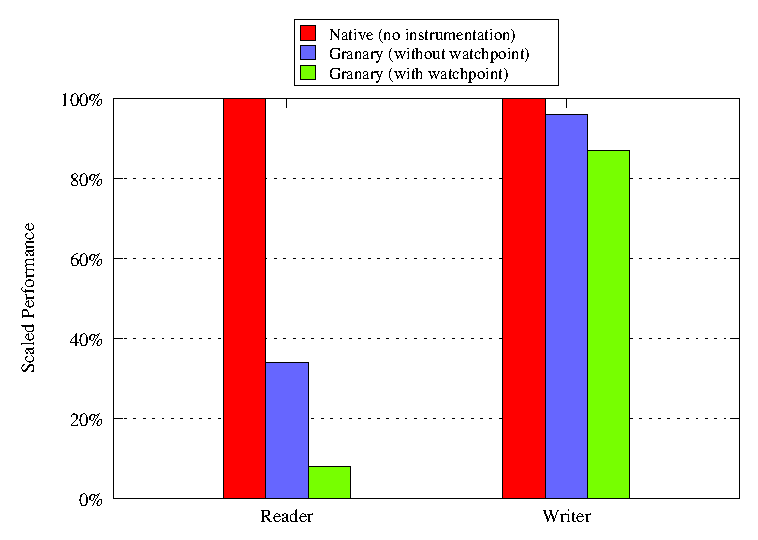
\includegraphics[width=0.45\textwidth]{performance}
\caption{Performance overhead for rcu torture test}\label{fig:perf}
\end{figure}
%We evaluated the performance of behavioural watchpoints using a microbenchmark and RCU torture test running with 100 readers and 5 writers. Our tests ran on a desktop equipped with an Intel\textregistered\ Core\texttrademark\ i7-860 2.80 GHz CPU, 8GB memory, and an Intel 82578DM Gigabit Ethernet card. Watchpoint instrumentation was enabled for every memory load and store, and watchpoints were active for all the RCU protected memory allocated from the memory pool.
We evaluated the performance of behavioural watchpoints using a microbenchmark and RCU torture. Our tests ran on a desktop equipped with an Intel\textregistered\ Core\texttrademark\ i7-860 2.80 GHz CPU, 8GB memory, and an Intel 82578DM Gigabit Ethernet card. Watchpoint instrumentation was enabled for every memory load and store, and watchpoints were active for all the RCU protected memory allocated from the memory pool.

\paragraph{Microbenchmark} The microbenchmark performed a tight-loop of memory operations on watched addresses and exhibits the worst-case performance overhead of watchpoints (about 20{\footnotesize$\times$}). This is expected because our instrumentation adds instructions to each memory load and store.
 %added to all memory returned from kernel heap allocators. 
%To evaluate the performance overhead incurred by the Granary and watchpoint we used rcutorture module running with 100 reader and 5 writer threads. As experimental setup, we run our system in Guest Virtual machine (QEMU) running with four core and powered with Linux 2.6.32 kernel on a Host system equipped with an Intel(R) Core(TM) i7-860, 2.80 GHz CPU. Our evaluation strategy involves running rcutorture module natively, under the control of Granary \& Granary with watchpoint active and studying the following parameters :
%\paragraph{\texttt{rcutorture}} We tested the \texttt{rcutorture} kernel module. It exhibited interesting behaviour: all threads experienced a minimum of 6{\footnotesize$\times$} overhead; however, readers were abnormally penalized and tended to see more stale data. We think this is because each writer synchronized with fewer readers.
%\paragraph{RCU tortute test} We tested the performance overhead incurred by Granary and watchpoints using \texttt{rcutorture} kernel module. Our evaluation strategy involves running rcutorture module natively, under the control of Granary \& Granary with active watchpoints and studying the following parameters :
\paragraph{RCU torture test} RCU torture is a kernel module which tests the
performance and correctness of RCU. We used this module to test the
performance overhead of Granary and watchpoints. The module was setup to
run with 5 updaters and a 100 readers. It was run
natively, under the control of Granary \& finally under
Granary with active watchpoints. We observed the following:
\begin{enumerate}
	\item[i)] The number of successful updates
	\item[ii)] The number of successful reads/
\end{enumerate}
%We recorded these parameters by running rcutorture module for 60 sec and averaged it over five different runs. Table~\ref{table:nonlin} below shows these parameters for three different cases. Our experimental result shows moderate decrease in ver number which shows the number of times writer task has changed the structure visible to readers but there is a drastic decrease in the readers \emph{Readers Pipe} and \emph{Readers batch} showing the increase in the readers seeing stale data. We think this is because each writer synchronized with fewer readers. The performance of readers and writers based on these parameters is shown in figure~\ref{fig:perf}.
We recorded these parameters by running rcutorture module for 60 sec and
averaged it over five different runs. Figure~\ref{fig:perf} shows the
results obtained. As can be seen, there is moderate decrease in the number
of updates and a drastic decrease in number of readers. This is because
where there was minimal overhead on the read critical section, we have
added additional instructions to instrument RCU.



% The result shows a moderate decrease in the performance of writer but the performance of readers decreases by approximately 10 times. One of the reason for this is we are testing the system with 100 readers but only 5 writers thread and read is the most frequent operation in the rcu torture test. Our system also instrument both memory read and write which is going to be costly but it gets amortized over the large number of instructions.

%\begin{table*}[thp!]
%\caption{Reader and Writer performance for rcu torture test}
% title of Table
%\centering
% used for centering table
%\begin{tabular}{c c c c}
% centered columns (4 columns)
%\hline\hline
%inserts double horizontal lines
%rcu-tortute-test & Ver & Reader-Pipe & Reader-Batch  \\ [0.5ex]
% inserts table
%heading
%\hline
% inserts single horizontal line
%Native(no instrumentation) & 2112 & 233093662 & 214069371 \\
% inserting body of the table
%Granary(without watchpoint) & 2043 & 87237464 & 83627748 \\
%Granary(with watchpoint) & 1850 & 16996975 & 16996075 \\[1ex]
% [1ex] adds vertical space
%\hline
%inserts single line
%\end{tabular}
%\label{table:nonlin}
% is used to refer this table in the text
%\end{table*}

%The other interesting observation we made is decrease in the performance overhead is not much because of watchpoint. There is significant drop in the performance of readers when rcutorture is run under the control of granary and watchpoint is not active. One reason for this is we annotated all rcu read side primitive to make a callback to kernel wrapper. These kernel wrapper runs natively and are not in code-cache. There is a cost involved when Granary switches execution from the code-cache to native since it has to switch the stack and save and restore the machine context. We have seen similar behaviour earlier with other file-system modules while running benchmarks like postmark~\cite{katcher97postmark} which involves many context switches. We have not yet verified this with rcutorture module.

The more interesting observation is that the decrease in performance
overhead is mainly caused due to Granary and not watchpoint. The
primary reason for this is that the rcu read critical section primitives
were annotated to make a callback into the wrapper. The kernel wrapper
runs natively and is not present in the code-cache. Switching execution
from code-cache to native has a performance impact since Granary has
to switch the stack, and save and restore the machine context. We have
seen similar behavior with file-system modules running other benchmarks
which involved many context switches. We are still to verify these
with RCU torture.

\subsection {RCU debugger}
To evaluate our system for rcu debugging, we introduced few rcu bugs violating
Rule 0, 1 and 2, as discussed in section ~\ref{sec:back}. Some examples of
these bugs are shown in Figures\textbf{AKSHAYTHEREISNORCUuseRule0figure}~\ref{RCUuseRule0},~\ref{fig:rcuderefbug} and~\ref{fig:rcuusebug}.
The first bug violated Rule 0 where the alias \emph{p} of RCU protected
date \emph{q} is referenced outside the read critical section. We
identify it by comparing the \emph{generation number} and watchpoint
\emph{generation number}. We find that the thread \emph{generation number}
is odd and not equal to the watchpoint \emph{generation number} at the
point of memory reference. The second bug we introduced violated Rule 1.
The RCU protected data \emph{q} was directly accessed without using
\emph{rcu\_dereference}. We notice at the time of access that the pointer
is a source and not an alias generated by \emph{rcu\_dereference}. This
is done by by checking \emph{meta\_info$\rightarrow$source}. We also notice
at this point that the \emph{generation number} and watchpoint \emph{generation number}
are not the same. We tesed Rule 3 violation by dereferencing RCU pointer in
a read critical section other than where it was aliased using \emph{rcu\_dereference}.
We tested this for a simple case where there is no recursive use of read critical
section. We identify this by checking both thread as well as generation
\emph{generation numbers}.

%To evaluate our system for rcu debugging, we introduced few rcu bugs violating Rule 0, 1 and 2, as discussed in section ~\ref{sec:back}. The details of the introduced bugs is provided in figure~\ref{fig:RCUuseRule0},~\ref{fig:rcuderefbug} and~\ref{fig:rcuusebug}. The first bug voilate Rule 0 where the alias \emph{p} of rcu protected data \emph{q} is getting referenced outside read critical section. Our system identified it by comparing the thread \emph{generation number} and watchpoint \emph{generation number}. Our system found the thread \emph{generation number} is odd and not equal to watchpoint \emph{generation number} at the point of memory reference. The second bug we introduced voilates Rule 1, where the rcu protected data \emph{q} is directly getting accessed without using \emph{rcu\_dereference()}. Our system noticed that when the memory gets accessed, the pointer is a source and not one of  alias generated by \emph{rcu\_dereference()} by checking \emph{meta\_info$\rightarrow$source}. Our system also noticed that at this point the thread \emph{generation number} and watchpoint \emph{generation number} is not same. We also tested the Rule 3 violation by dereferncing rcu pointer in read critical section other than the one where it gets alias using \emph{rcu\_dereference()}. We tested this for simple case where there is no recursive use of read critical section. Our system identifies this by checking both thread \emph{generation number} and watchpoint \emph{generation number}. 

%We evaluated our system by introducing simple bugs in rcutorture module and found that it catches the violation of three rules mentioned in section~\ref{sec:back}. There is need to test the system with complex rcu bugs which includes the voilation of more than one rules and corner cases. We are hopeful that our system will be able to catch such bugs also.

We evaluated our system by introducing simple bugs in rcutorture module and
found that it detects the violation of three rules mentioned in
section~\ref{sec:back}. There is need to test the system with complex rcu bugs
which violate multple rules and corner cases. We expect
that our system will be able to catch most of these bugs.


\subsection{Space Overhead}
The size of shadow memory depends on the number of watchpoints added and currently active. Shadow memory is used to store the meta-information, the size of which is proportional to the number of threads running. This increases the space overhead and makes it \emph{M x N} for the system running \emph{N} threads and having \emph{M} active watchpoint. The point to be noted that this is the virtual memory overhead. We do not expect the space overhead to be serious concern on a 64 bit architecture.    




\section{Related Work}\label{sec:related}
Application debugging is a necessary part of software development cycle. There are many software, hardware and hybrid technique exists for debugging. The importance of such debugging technique increases as the complexity of software increases. Read Copy Update (RCU) is one of the synchronization technique which is heavily used in the linux kernel because of its lightweight read-side overhead. Programming of software system using RCU is complex and often lead to bugs due to its incorrect usage. Debugging such incorrect usage of rcu primitive is challenging as one needs to follow many rules \& assumptions to verify its correct usage. 

\subsection{RCU debugging}
There are many existing solution which is used for analysing the incorrect usage of RCU synchronization primitive. Sparse~\cite{sparse} is one of the existing tool which uses static analysis method to verify the correct usage of RCU. It uses \emph{\_\_rcu} tag to annotate the RCU protected pointers and flags traversals of RCU-protected pointers that are not properly protected either by an RCU read-side critical section or an update-side lock. One of the demerits of using sparse is its output gets heavily ridden with false positives, requiring more time and effort to interpret. Lockdep-RCU is another method which is used for analysing the incorrect usage of \emph{rcu\_derefence()}. It emits a runtime error if they gets executed outside of an RCU read-side critical section. One of the important limitation with Lockdep-RCU~\cite{PaulEMcKenney2010LockdepRCU} solution is it catches only the incorrect usage of \emph{rcu\_derefence()} and \emph{rcu\_assign\_pointer()}. 

\subsection{Watchpoint}
Watchpoint is an important debugging facility that helps developers track the memory references. Almost all the hardware state-of-the-art processor provides support for limited hardware watchpoints. There has been several proposal in the past on implementing software watchpoint and some of them using methods of Dynamic Binary Instrumentation(DBI).
%makes the case for supporting an unlimited number of watchpoints. A hardware solution is proposed and multiple applications are described. Unlike our approach, the cited approach depends on specialised hardware and requires that applications using these watchpoints maintain their own context-specific information.
%In , 
\paragraph{Software-based}
Zhao \emph{et al.}~\cite{Zhao:2008} describe a method of implementing an efficient and scalable DBT-based watchpoint system. His method uses page protection and indirection through a hash table to track watched memory. This approach does not support watching ranges of memory, nor does it support context-specific information. Lueck \emph{et al.} \cite{PinADX} introduce semantic watchpoints as part of the PinADX system, an extension of the PIN DBT framework. PinADX enables interactive debugging by triggering debugger breakpoints when semantic conditions are met. While similar in spirit to behavioural watchpoints, semantic watchpoints do not maintain context-specific, per-watchpoint state. Wahbe \emph{et al.}~\cite{Wahbe:1992} also proposes the implementation of software watchpoint using code patching and static analysis.  Another interesting approach proposed by keppel \emph{et al.}~\cite{Keppel:93a} to use checkpoint for memory updates. But one of the important thing about all of these works is they are only valid for userspace. The latest patches of MemCheck in Valgrind~\cite{Seward:2005} also provides the support of adding watchpoint. They uses link-list to maintain the watchlist. This puts a sevear restriction on their performance.   

\paragraph{Hardware-based}
Greathouse \emph{et al.}~\cite{UnlimitedWatchpoints} propose a hardware solution that efficiently supports an unlimited number of watchpoints. Witchel and Asanovic \cite{Mondrix} describes the implementation of memory protection domains for the Linux kernel. Protection domains are implemented using specialised hardware and enable fine- and coarse-grained memory protection using a mechanism similar to hardware watchpoints. Unlike our approach, both \cite{Mondrix} and \cite{UnlimitedWatchpoints} depend on specialised hardware and require that applications using this hardware  separately maintain context-specific information. Suh \emph{et al.} \cite{SecureProgramExecFlowTracking} proposes a method of secure program execution by tracking dynamic information flow. Memory tagging at the hardware level allows their system to track tainted data as it propagates through a running program. Behavioural watchpoints are similar insofar as a watched address is tagged, and this tag propagates through a program.


\section{Conclusions}\label{sec:conclusions}
Read-copy update (RCU) is a synchronization mechanism that gets heavily used in the linux kernel. It improves scalability by allowing readers to execute concurrently with writers. RCU ensures read coherence by maintaining multiple versions of data structures and ensuring that they are not freed until all pre-existing read-side critical sections complete. Using RCU for developing parallel system is complicated and requires lot of care. The user need to follow many rules or assumption and incorrect usage of rcu leads to programming bugs. These bugs are hard to debug. There are existing solution mention in section which deals with the incorrect usage of RCU but they are imprecise and cause many false positive.  In this project we are trying to analyse the incorrect usage of RCU violating three rules mentioned in section~\ref{sec:proposal}. Our system uses \emph{Watchpoint} mechanism implemented using Dynamic Binary Instrumentation (DBI) technique to track the references of RCU protected data. \emph{Watchpoint} mechanism provides us infrastructure to track the memory references and gives us callback on the access of RCU protected data which is used to verify the access policy. The algorithm we used to implement the policy is simple and uses thread and watchpoint \emph{Generation number} to check the policy.  Our system updates \emph{Generation number} when it encounters rcu primitive. Our system currently enforces simple policies and is limited to classical RCU only. 


\section{Acknowledgements}
We are indebted to Professors Ashvin Goel and Angela Demke Brown who
guided us through this project. We are also extremely grateful to the
rest of the DynamoRio-Kernel group for the extended discussion and
assistance while debugging. We are also grateful to Dr Paul E. McKenney
for his valuable input in deciding the goals of this project. Finally
we are also extremely grateful to Professor Cristiana Amza for offering
this course and allowing us to pursue this project.

\bibliography{db}
\bibliographystyle{abbrv} 

\end{document}

